% !TEX encoding = UTF-8 Unicode
%!TEX root = memoria.tex
% !TEX spellcheck = es-ES
%%=========================================
\chapter{Estado del arte}
%%=========================================

\section{Neuroimagen}

Las técnicas de neuroimagen han cambiado el panorama en que los científicos abordan las hipótesis sobre la anatomía funcional del cerebro, especialmente en relación con el comportamiento y los trastornos clínicos. \cite{bold_fmri}

\subsection{Anatomía básica del cerebro}

El cerebro humano está compuesto por alrededor de $10^{11}$ \hyperref[eda:neurona]{neuronas} y sobre $10^{4}$ sinapsis por cada neurona comprimidas en un volumen de unos $1,400cm^{3}$.

\begin{figure}[H]
  \centering
    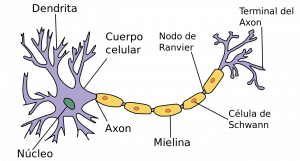
\includegraphics[scale=0.75]{img/neurona.png}
  \caption{Neurona cerebral}\label{eda:neurona}
\end{figure}

Las neuronas están densamente conectadas y tienen muchas \hyperref[eda:neurona]{dentritas}. Asi mismo los axones conducen las señales electricas y están recubiertos por mielina. La mielina es un factor determinante a la hora de establecer la señal y el contraste de la resonancia magnética. Las neuronas se organizan en tres tipos de \hyperref[eda:tejidos]{tejidos}:

\begin{itemize}
	\item Sustancia Gris (GM): Contiene numerosos cuerpos celulares (somas) y relativamente pocos axones cubiertos de mielina. Se asocia con la función del procesamiento de la información, es decir con la capacidad del razonamiento. Se localiza en la superficie del cerebro, formando la corteza cerebral, que corresponde con la organización mas compleja de todo el sistema nervioso.
	\item Sustancia Blanca (WM): Principalmente está formado por un gran número de axones(parte de la neurona encargada de transmitir l información) cubiertos de mielina y contiene relativamente pocos cuerpos celulares. Se corresponde con la parte interior del cerebro.
	\item Fluido Cerebroespinal (CSF): Para la protección mecánica básica e inmunológica del cerebro.
\end{itemize} 

\begin{figure}[H]
  \centering
    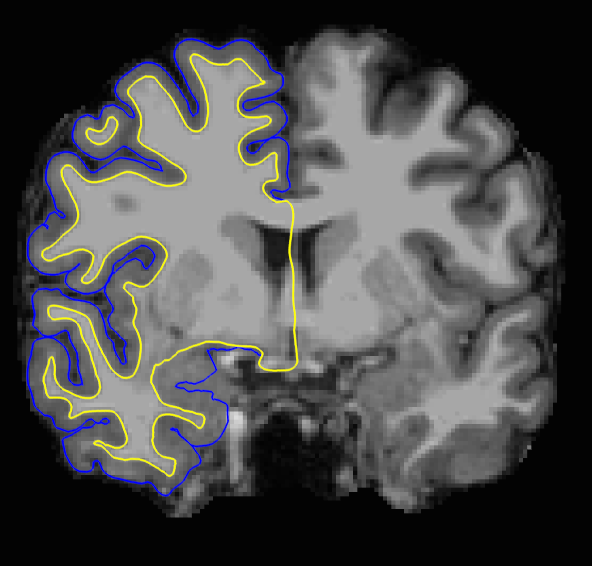
\includegraphics[scale=0.60]{img/tejidos.png}\label{eda:tejidos}
  \caption{El cerebro requiere el 20\% de la energía total del cuerpo y entre el 60 y 80\% de esta energía es utilizada en las conexiones cerebrales (comunicación entre neuronas)}
\end{figure}

\cite{brainhack}

\section{Datos del cerebro}

El campo de la neuroimagen incluye el uso directo o indirecto de varias técnicas de imagen estructural o funcional del cerebro.

Los datos anatómicos o \hyperref[eda:anat]{imagen} anatómica describen el tamaño, la forma y la integridad de las estructuras de los tejidos en el cerebro. Se obtiene al realizar una resonancia magnética convencional y nos permite visualizar de manera contrastada la sustancia gris y la sustancia blanca.

\begin{figure}[H]
  \centering
    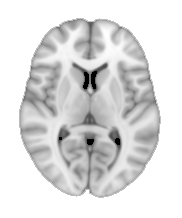
\includegraphics[scale=0.75]{img/anat.png}
  \caption{Imagen estructural del cerebro}\label{eda:anat}
\end{figure}

Los datos \hyperref[eda:func]{funcionales} calculan los patrones de activación de las diferentes poblaciones de neuronas o regiones dentro del cerebro. Permite detectar zonas de mayor oxigenación en el cerebro cuando el paciente está realizando una actividad o en estado de reposo.

\begin{figure}[H]
  \centering
    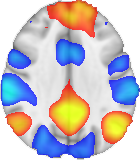
\includegraphics[scale=0.75]{img/func.png}
  \caption{Imagen funcional del cerebro}\label{eda:func}
\end{figure}
\cite{brainhack,fmri_oxford}

\subsubsection{Datos funcionales}

Mide la actividad neuronal a través de la señal dependiente del nivel de oxigenación de la sangre de cada voxel (\hyperref[glos:bold]{BOLD}). La actividad neuronal causa una mayor demanda de energía, a través de un proceso llamado respuesta hemodinámica la sangre libera oxigeno a las neuronas activas, disparadas a una tasa mucho mayor en comparación con las neuronas inactivas. \cite{brainhack,bold_fmri}

\begin{figure}[H]
  \centering
    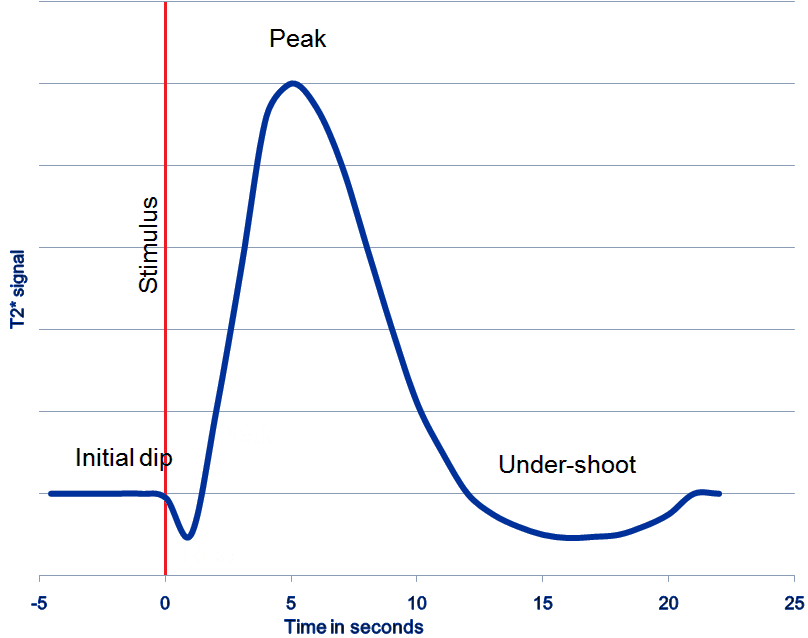
\includegraphics[scale=0.5]{img/bold.png}
  \caption{Respuesta hemodinámica}
  \label{eda:bold}
\end{figure}

Mientras que la actividad neuronal ocurre en milisegundos, la respuesta hemodinámica es más lenta y toma alrededor de 5 segundos en alcanzar su máximo como se puede ver en la figura \ref{eda:bold} seguido por un descense inferior al nivel basal aproximadamente a los 15 segundos.

En la mayoría de las aplicaciones la resolución espacial se encuentra entre 1 y 5mm. La resolución temporal suele estar entre 0.5 y 3 segundos ~\ref{eda:resol}.\cite{courserafmri1,brainhack,fmri_oxford}

\begin{figure}[H]
  \centering
    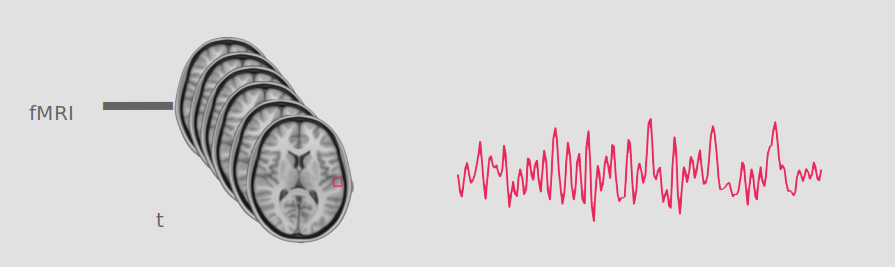
\includegraphics[scale=0.5]{img/resol.png}
  \caption{Resolución temporal}
  \label{eda:resol}
\end{figure}

Existen dos modalidades principales de fMRI:

\begin{itemize}
	\item \textbf{Task fMRI}: El sujeto realiza una tarea durante el escaner
	\item \textbf{Rest fMRI}: El sujeto se encuentra relajado y no hace ni piensa en nada durante el escaner.
\end{itemize}

El presente experimento se obtiene un conjunto de datos basado en la segunda modalidad.

\section{Estandar de imágen médica: DICOM}

Del Inglés \textit{Digital Imaging and Communications in Medicine} fué creado por \textit{National Electrical Manufacturers and Association} para permitir la visualización y distribución de imágenes médicas. Es el estandar mundialmente reconocido para este fin.\cite{dcm2nifti}

DICOM tiene un conjunto muy amplio de servicios, la mayoría de los cuales implica transmisión de datos sobre la red, y el formato de fichero en que se sustenta es en realidad una ampliación posterior y de menor importancia del estándar. Queda recogido en el PS3.10 \cite{dicom} del estandar.\cite{nema}

Un único archivo DICOM contiene la cabecera, la cual contiene información sobre el nombre del paciente, el tipo de escaner, la dimensión de la imágen y otros metadatos, además de todos los datos de la imágen en formato binario. Es posible comprimirlo a fin de reducir el tamaño de la imágen. A menudo son separados en \textit{slices} de dos dimensiones, pero pueden ser combinadas en un único archivo.\cite{dcm2nifti}


\subsection{Cabecera DICOM}

La siguiente \hyperref[dicom:dummy_image]{imagen} muestra un hipotético archivo DICOM. En este ejemplo, los primeros $794$ bytes son usados para la cabecera DICOM, la cual informa de la dimensión de la imágen y guarda otra información sobre el escaner. El tamaño de la cabecera puede variar en función de cuanta informaión se almacena en ella. En este caso se encuentra una imagen de $109x91x2$ voxels, con una resolución de un byte por voxel (por tanto el tamaño total de la imagen es de 19838 bytes). La imagen se encuentra a continuación de los datos de la cabecera, generalmente en el mismo archivo.

\begin{figure}[H]
  \centering
    \label{dicom:dummy_image}
    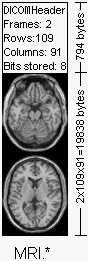
\includegraphics[scale=0.75]{img/dcmi.png}
  \caption{Imagen estandar  DICOM}
\end{figure}

El estandar de almacenamiento que recoge DICOM, reserva los 128 primeros bytes para el preambulo(el cual generalmente no contiene información, son todo ceros) segido por los caracteres `D', `I', `C' y `M'. Tras estos caracteres aparece la información de la cabecera, la cual se organiza en ``grupos''. Por ejemplo el grupo \textit{002hex} en la siguiente \hyperref[dicom:dummy_header]{imagen} es el grupo de los metadatos del archivo, en el siguiente ejemplo contiene tres elementos: uno define la longitud del grupo, otro guarda la versión del archivo y el tercero almacena la sintaxis de transferencia.

\begin{figure}[H]
  \centering
    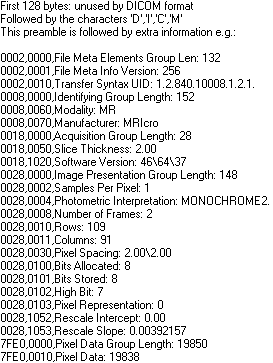
\includegraphics[scale=0.75]{img/header.png}
  \caption{Cabecera  DICOM}\label{dicom:dummy_header}
\end{figure}

Los elementos requeridos dependen del tipo de imagen, en la parte 3 del archivo DICOM de ejemplo en la imagen \ref{dicom:dummy_header} aparece como `MR' (0008:0060), por tanto tendrá que contener los elementos que describen un \textbf{MRI}. La ausencia de este elemento supone una violación del estandar.

Un elemento de particular importancia es \textbf{002:0010} (ver la tabla \ref{dicom:tab_sintaxis}), el cual define el identificador único de transferencia de sintaxis \textbf{Transfer Syntax Unique Identification}. Este valor informa la estructura de los datos de la imagen, revelando si los datos han sido comprimidos o no (lo que podría suponer perdidas en los datos de altas frecuencias).

\begin{table}[H]
  \centering
    	\tiny
  \begin{tabular}{|c|l|}
    % body of tabular environment 
    \hline
    Transfer Syntax UID	& Definition \\
    \hline
    1.2.840.10008.1.2.x	& Raw data, Eplicit VR x = 1: Little Endian x = 2: Big Endian \\
	1.2.840.10008.1.2.4.xx &	JPEG compression xx = 50-64: Lossy JPEG xx = 65-70:Lossless JPEG \\
	1.2.840.10008.1.2.5	& Lossless Run Length Encoding  \\
    1.2.840.10008.1.2 		&	Raw data, Implicit VR, Little Endian \\	
    1.2.840.10008.1.2.4.xx & JPEG compression xx = 50-64: Lossy JPEG xx = 65-70: Lossless JPEG \\
    1.2.840.10008.1.2.5 & Lossless Run Length Encoding \\
    \hline
  \end{tabular}
  \caption{Definición de transferencia de sintáxis}\label{dicom:tab_sintaxis}

\end{table}

Además de informar sobre la técnica de compresión (si existe), el \textbf{UID} de la sintaxis de transferencia infroma del orden de los bytes de datos sin procesar. Cada host puede almacenar de forma diferente los valores \textbf{integer} (big endian y little endian ordering). Si consideramos un entero de 16 bits con el valor 257: el byte más significativo almacena el valor 01 (= 255), mientras que el byte menos significativo almacena el valor 02. Algunas computadoras guardarán este valor como 01:02, mientras que otras lo almacenarán Como 02:01. Por lo tanto, para los datos con más de 8 bits por muestra, un visor DICOM puede necesitar cambiar el orden de bytes de los datos para que coincida con el orden utilizado por el equipo.

\section{Estandar de imágen médica: NIFTI}

Como se ha mencionado con anterioridad, el estandar DICOM provee de un marco de trabajo para transferir, almacenar e imprimir imágenes médicas. Mientras este formatos es muy flexible y comprensible, requiere de un gran esfuerzo y es costoso de implementar. Sin embargo, para investigar sobre estas imágenes es suficiente con un formato mucho más sencillo que almacena unicamente los metadatos más relevantes.\
Al contrario que DICOM, NIfTI es un formato muy simple. Este formato ha sido ampliamente aceptado en el campo de la invesigación de neuroimagen, permitiendo combinar diferentes herramientas de analisis y procesado, desarrollada por distintos equipos.

\subsection{Cabecera}

Hereda su estructura de 348 bytes del formato estandar \textbf{ANALYZE}. En los últimos cuatro bytes de la cabecera se corresponden con el campo ``mágico'' que indica si la cabecera y la imagen están en un único archivo ($magic = n+1|0$) o en dos separados ($magic = ni1|0$). Añade cuatro bytes adicionales al formato \textbf{ANALYZE} indicando la \textit{extensión} de la cabecera. Por defecto esos cuatro bytes son ceros.
La imagen y la cabecera pueden ser almacenados en ficheros distintos usando las extensiones .hdr y .img, o en un único archivo con la extensión .nii donde la cabeceraocupa los primeros 348 bytes y los datos de la imagen suelen ocupar a partir del byte 352.

%%=========================================
\section{Neuroimagen de temblor esencial}

El temblor esencial (\hyperref[glos:et]{ET}) es uno de los desordenes neurológicos más comunes con una prevalencia del 0.9\% en la población general, que incrementa con la edad y que puede afectar a las extremidades, la cabeza, el cuello, la voz o varias combinaciones, con una estimación de aproximadamente 5\% sobre los individuos de 65 años. El comienzo clinico es bimodal, algunos de los sintomas se presentan en una fase muy temprana de la vida, mientras otros sintomas se presentan en una fase más tardía. \cite{movedisorder,ethandbook,anderson}

Algunos estudios recientes sugieren que se trata de un proceso de evolución lenta degenerativa con sintomas que no están relacionados con el sistema motor como disfunciones cognitivas, ansiedad, depresión y perdida de audición.
El diagnóstico clínico suele realizarse basado en el historial médico y los resultados de un examen neurológico. \cite{movedisorder}

\subsection{Fisiopatología}

La fisiopatología del ET no se encuentra completamente entendida, pero algunos estudios clínicos y de imagen apuntan a que el cerebelo está involucrado. Se define como un acción de temblor con una frecuencia entre 4 y 8 Hz \cite{anderson}, en reposo, sin ningun otro trastorno neurológico.
Algunos estudios neurológicos y de animales,post-mortem, indican que la oliva inferior, el cerebelo, el núcleo rojo, el tálamo y el cortex y sus neurotransmisores están involucrados. Estas areas conforman la red conocida como \hyperref[te:cerebelo-talamo-cortex]{cerebelo-tálamo-corticales} (CTC).\cite{rolectc,neuessentialsinet, anderson}

\begin{figure}[H]
  \centering
    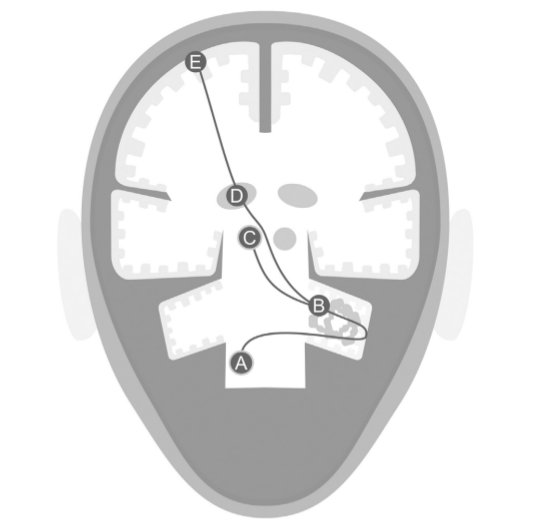
\includegraphics[scale=0.5]{img/cerebelo-talamo-cortex.png}
  \caption{Red del temblor: A)Oliva inferior; B) Núcleo dentado; C)Núcleo rojo; D)Tálamo; E) Cortex-motor} Imágen extraida de \cite{neuessentialsinet}    \label{et:cerebelo-talamo-cortex}
\end{figure}

Los estudios individuales basados en imágen estructural no han revelado anomalías significativas en pacientes con temblor esencial. Si embargo, estudios patólogicos más avanzados han mostrado cambios estructurales \cite{neuessentialsinet, anderson}.

\subsection{Imagen de Resonancia Magnética Funcional: fMRI}

La definición clínica de esta emfermedad se encuentra aún bajo debate. El diagnóstico clínico actual basado en la declaración de consenso de la Sociedad de Trastornos del Movimiento tiene un margen de error estimado del 37\% de los falsos positivos.\cite{neuessentialsinet}

Las técnicas de neuroimagen podrían reducir potencialmente el margen de error en los diagnósticos al obtener información sobre la patología cerebral subyacente y, en última instancia, podrían utilizarse como una herramienta de diagnóstico válida
Los estudios de imagen funcional son capaces de asociar el temblor esencial con la actividad cerebral en reposo o mientras realiza una actividad \cite{neuessentialsinet}. Las técnicas más comunmente utilizadas en fMRI basan sus estudios en el principio de cambios de contraste \hyperref[glos:bold]{BOLD}. Estas técnicas utilizan las diferentes propiedades magnéticas de la oxigenación y desoxigenación de la hemoglobina con el fin de identificar cambios en el flujo de sangre en las regiones del cerebro. Los cambios BOLD durante los movimientos voluntarios se asocian principalmente con la activación de la corteza sensimotora contralateral, las regiones subcorticales y el cerebro ipsilateraljunto con las desactivación significativa de las regiones subcorticales de la corteza sensimotora ipsilateral y el cerebelo contralateral \cite{movedisorder}.
Hasta la fecha hay pocos estudios basados en fMRI que evalúen los cambios \textbf{BOLD} relacionados con \textbf{ET}. Los sujetos con ET que manifestaron temblores durante el fMRI no solo muestran activación de estas areas, si no también aquellas que componen la red cerebelo-talamo-cortical en la imagen \ref{et:cerebelo-talamo-cortex}. 

Los artefactos generados durante la tarea son algunas limitaciones en este tipo de resonancias, a la hora de analizar la aparición de los sintomas del temblor esencial en un espacio confinado de un escaner MRI. Se pueden generar confusiones adicionales al intentar comparar los temblores involuntarios que aparecen en individuos con ET, con controles que a menudo se les pide imitar temblores. Se puede evitar la generación  estos artefactos (\textit{confounds} en inglés) realizando el estudio en estado de reposo \cite{ethandbook,movedisorder}. 

%%=========================================
\section{Preprocesado de neuroimágen}

El pipeline de preprocesado de neuroimagen depende generalmente del investigador, que métodos y en qué orden aplicar dichos métodos entre los siguientes:

\begin{itemize}
	\item Eliminación de los primeros volumenes para corregir el efecto de la saturación magnética (los primeros volumenes suelen tener una mayor intensidad). Algunas máquinas de MR ya lo realizan de forma automática.
	\item Slice Timing Correction (fMRI)
	\item Motion Correction (fMRI)
	\item Artifact Detection (fMRI)
	\item Coregistro
	\item Normalización
	\item Smoothing o suavizado
	\item Filtro de pasa banda: aunque existe controversia está ampliamente aceptado el filtrado entre las frecuencias 0.01 y 0.08 Hz en estudios fMRI en estado de reposo.\cite{brainhack}
	\item Segmentación en regiones de interés (sMRI) 
	\item Extracción del cerebro (sMRI)
\end{itemize}

\subsection{Conversión DICOM a NIfTI}

La mayoría de las herramientas más conocidas para el procesado y visualización de imagen médica, todavía no son compatibles con el formato DICOM, requieren que las imágenes estén almacenadas en formato \textbf{NIfTI}, sin embargo las imágenes capturadas por los escaneres actuales almacenan estas imagenes bajo el estandar DICOM.
Dicho esto, el primer paso en cualquier flujo de preprocesado suele consistir en convertir las imágenes DICOM en imágenes NIfTI. Esta tarea no siempre es sencilla ya que el estandar DICOM es particularmente complicado y diferentes escaneres pueden extender de forma diferente el estandar, dando lugar a información diferente e incluso duplicada \cite{dcm2nifti}. Debido a esto nos encontramos incompatibilidades con el software que puede haber sido diseñado para su uso con un pequeño subconjunto de imágenes DICOM y por tanto mientras una herramienta de conversión funciona para unas imágenes, podría no hacerlo para otras.

\subsection{Extracción del cerebro}

Se trata del preproceso previo al registro y a la segmentación. Elimina los tejidos no cerebrales a fin de obtener mejores resultados en los pasos posteriores. Por ejemplo al registrar las imágenes funcionales en imágenes anátomicas de alta resolución. Las imágener fMRIsuelen tener muy pocos tejidos no cerebrales debido a la naturaleza de la imagen, sin embargo las imágenes MR de alta resolución a menudo tiene una gran cantidad de estos tejidos, como los ojos, la piel, grasa, músculo...etc y la robusted del algoritmo de registro depende en gran medida de la eliminación de estos tejidos \cite{bet}.

\begin{figure}[H]
  \centering
    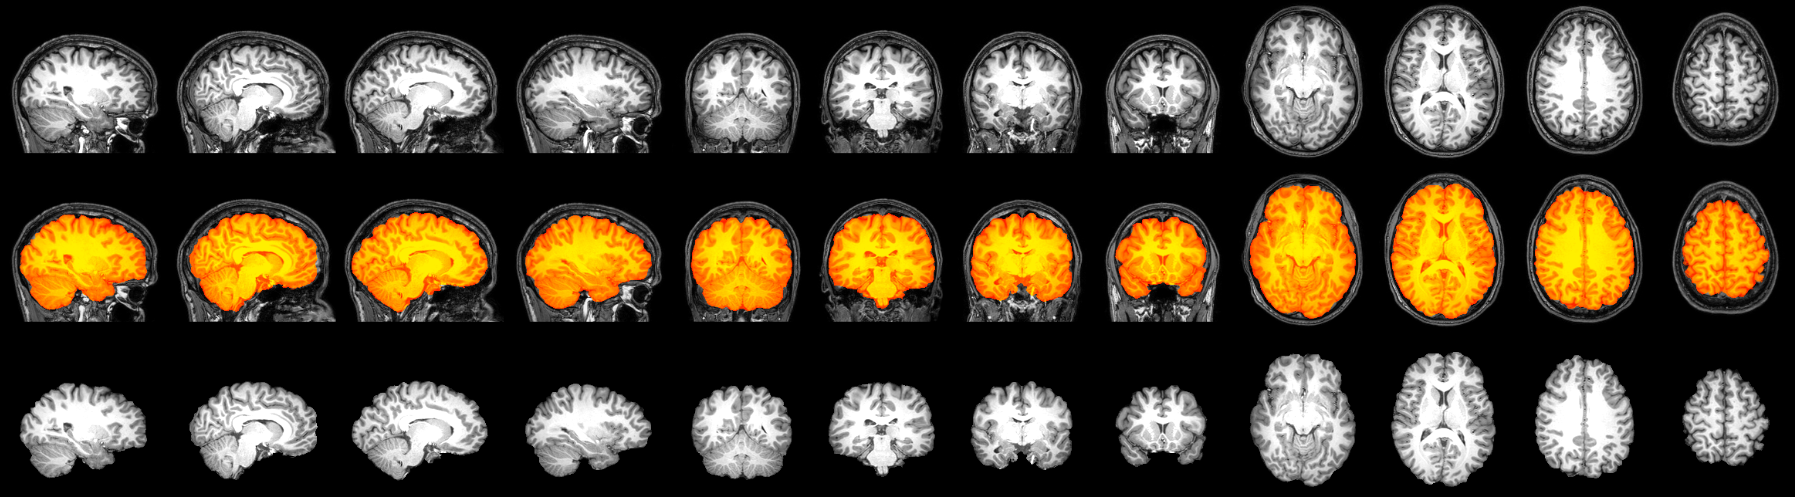
\includegraphics[scale=0.5]{img/skull_strip.png}
  \caption{Extracción del cerebro}         \label{preproc:skull_strip}
\end{figure}

Generalmente se elemina el fondo de la imagen para analizar los \textit{slice} de voxels.

\subsection{Segmentación}

\begin{figure}[H]
  \centering
    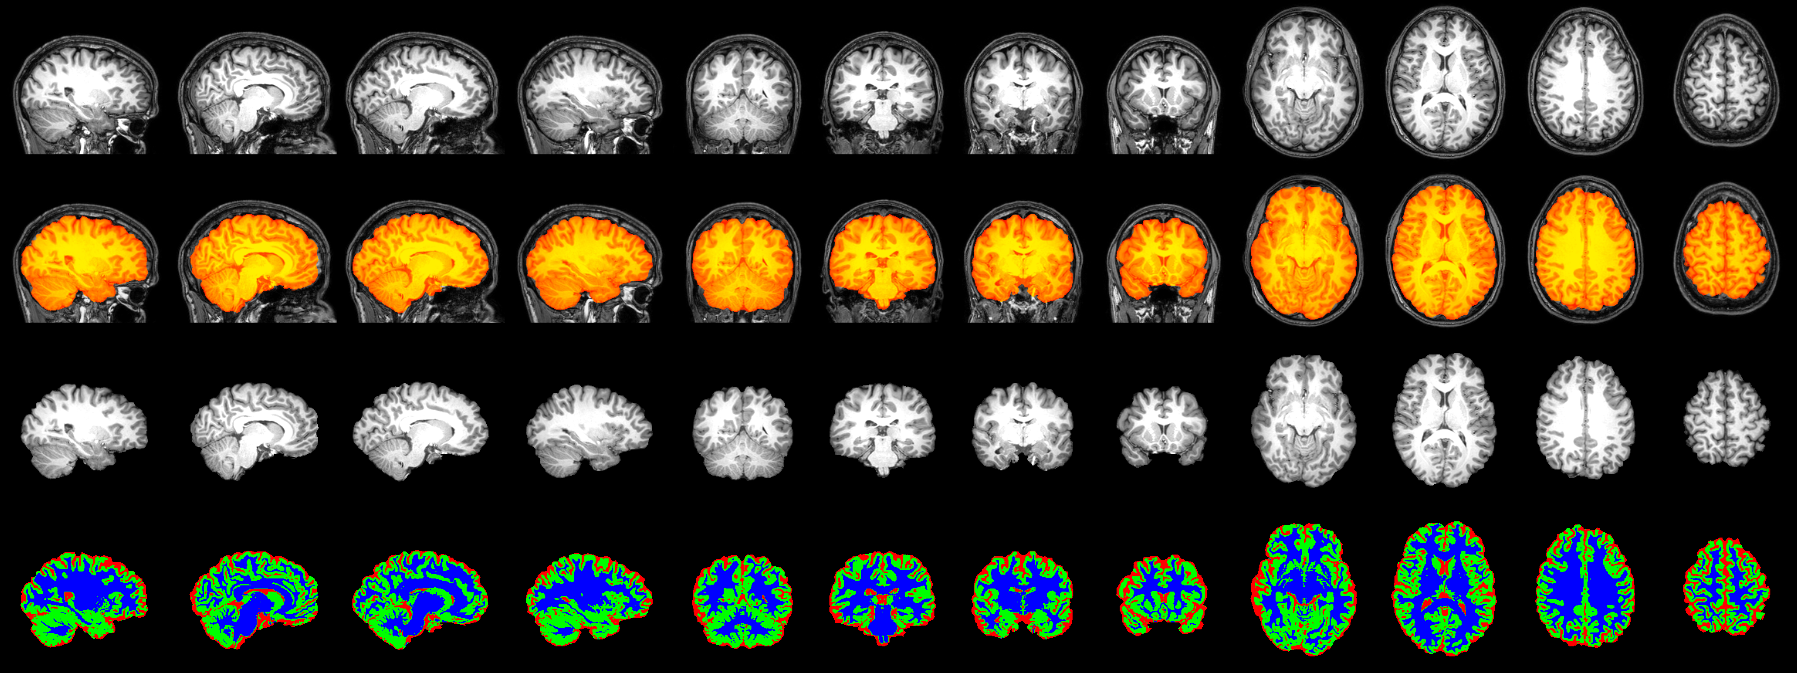
\includegraphics[scale=0.5]{img/segmentation.png}
  \caption{Segmentación de imagen T1}         \label{preproc:segmen}
\end{figure}

\subsection{Slice Timing Correction}

Dado que en las secuencias fMRI no se obtienen las \textit{slice} de un volumen en el mismo instante de tiempo, es necesario tener en cuenta las diferencias temporales de la adquisición. Por ejemplo si obtenemos un volumen con 25 slices en orden ascendente y cada una de ellas se capta cada 100 ms, hay una diferencia de 2.5 segundos entre la primera y la última. Es necesario conocer el orden de la adquisición para poder aplicar la corrección correctamente. Son tipicamente captadas utilizando uno de los siguientes tres métodos:
\begin{itemize}
	\item orden descendente (top-down)
	\item orden ascendente (bottom-up)
	\item intervalos
\end{itemize}

Slice Timing Correction se utiliza para compensar las diferencias de tiempo entre las adquisiciones de corte mediante la interpolación temporal de los cortes de modo que el volumen resultante sea casi equivalente a la adquisición de toda la imagen del cerebro en un solo punto de tiempo.


\begin{figure}[H]
  \centering
    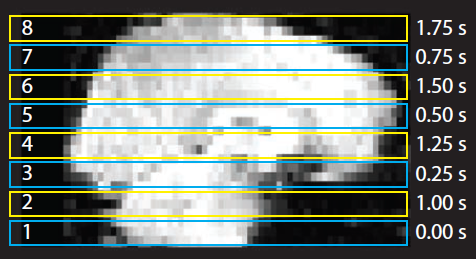
\includegraphics[scale=0.5]{img/slice_timming.png}
  \caption{Diferentes slides de un volumen 3D}         \label{preproc:slice_timming}
\end{figure}

\subsection{Corrección de movimiento}

También conocido como realineado, es usado para corregir los movimientos de la cabeza durante la adquisición de la imágen de datos funcionales, dado que incluso los pequeños movimientos de la cabeza condicen a la variación indeseada de los voxel y reducen la calidad de los datos. Con la corrección del movimiento se busca minimizar la influencia de los movimientos, registrando cada uno de los volumenes con un volumen de referencia. Este volumen de referencia suele ser la media de todos los puntos de tiempo.
El movimiento de la cabeza se puede caracterizar por seis parámetros, tres de traslación a lo largo de los tres ejes $X, Y, Z$ y tres de rotación con el centro en los mismos ejes.
Generalmente se realiza mediante una transformación afín de cuerpo rígido para transformar los datos con esos seis grados de libertad.

\begin{figure}[H]
  \centering
    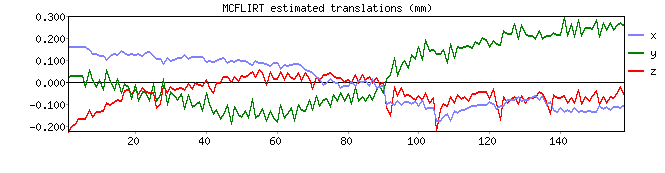
\includegraphics[scale=0.5]{img/tras.png}
  \caption{Corrección del movimiento de rotación}         \label{preproc:tras}
\end{figure}

\begin{figure}[H]
  \centering
    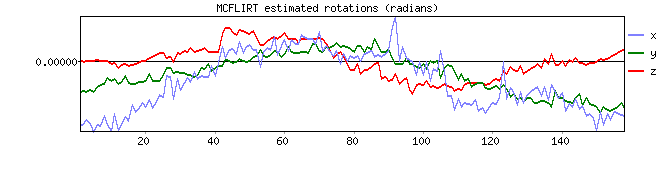
\includegraphics[scale=0.5]{img/rot.png}
  \caption{Corrección del movimiento de traslación}         \label{preproc:rot}
\end{figure}

\subsection{Detección de artefactos}

El movimiento de la cabeza altera sistemáticamente las correlaciones de la conectividad funcional en imágenes es estado de reposo. Casi ningún sujeto permanece inmovil, se puede observar en la imágen como algunos se mueven drasticamente, este movimiento se puede apreciar por el pico tan agudo que aparece en la gráfica. Un movimiento tan severo y repentino puede influir en los resultados finales del experimento. \cite{arts}

\begin{figure}[H]
  \centering
    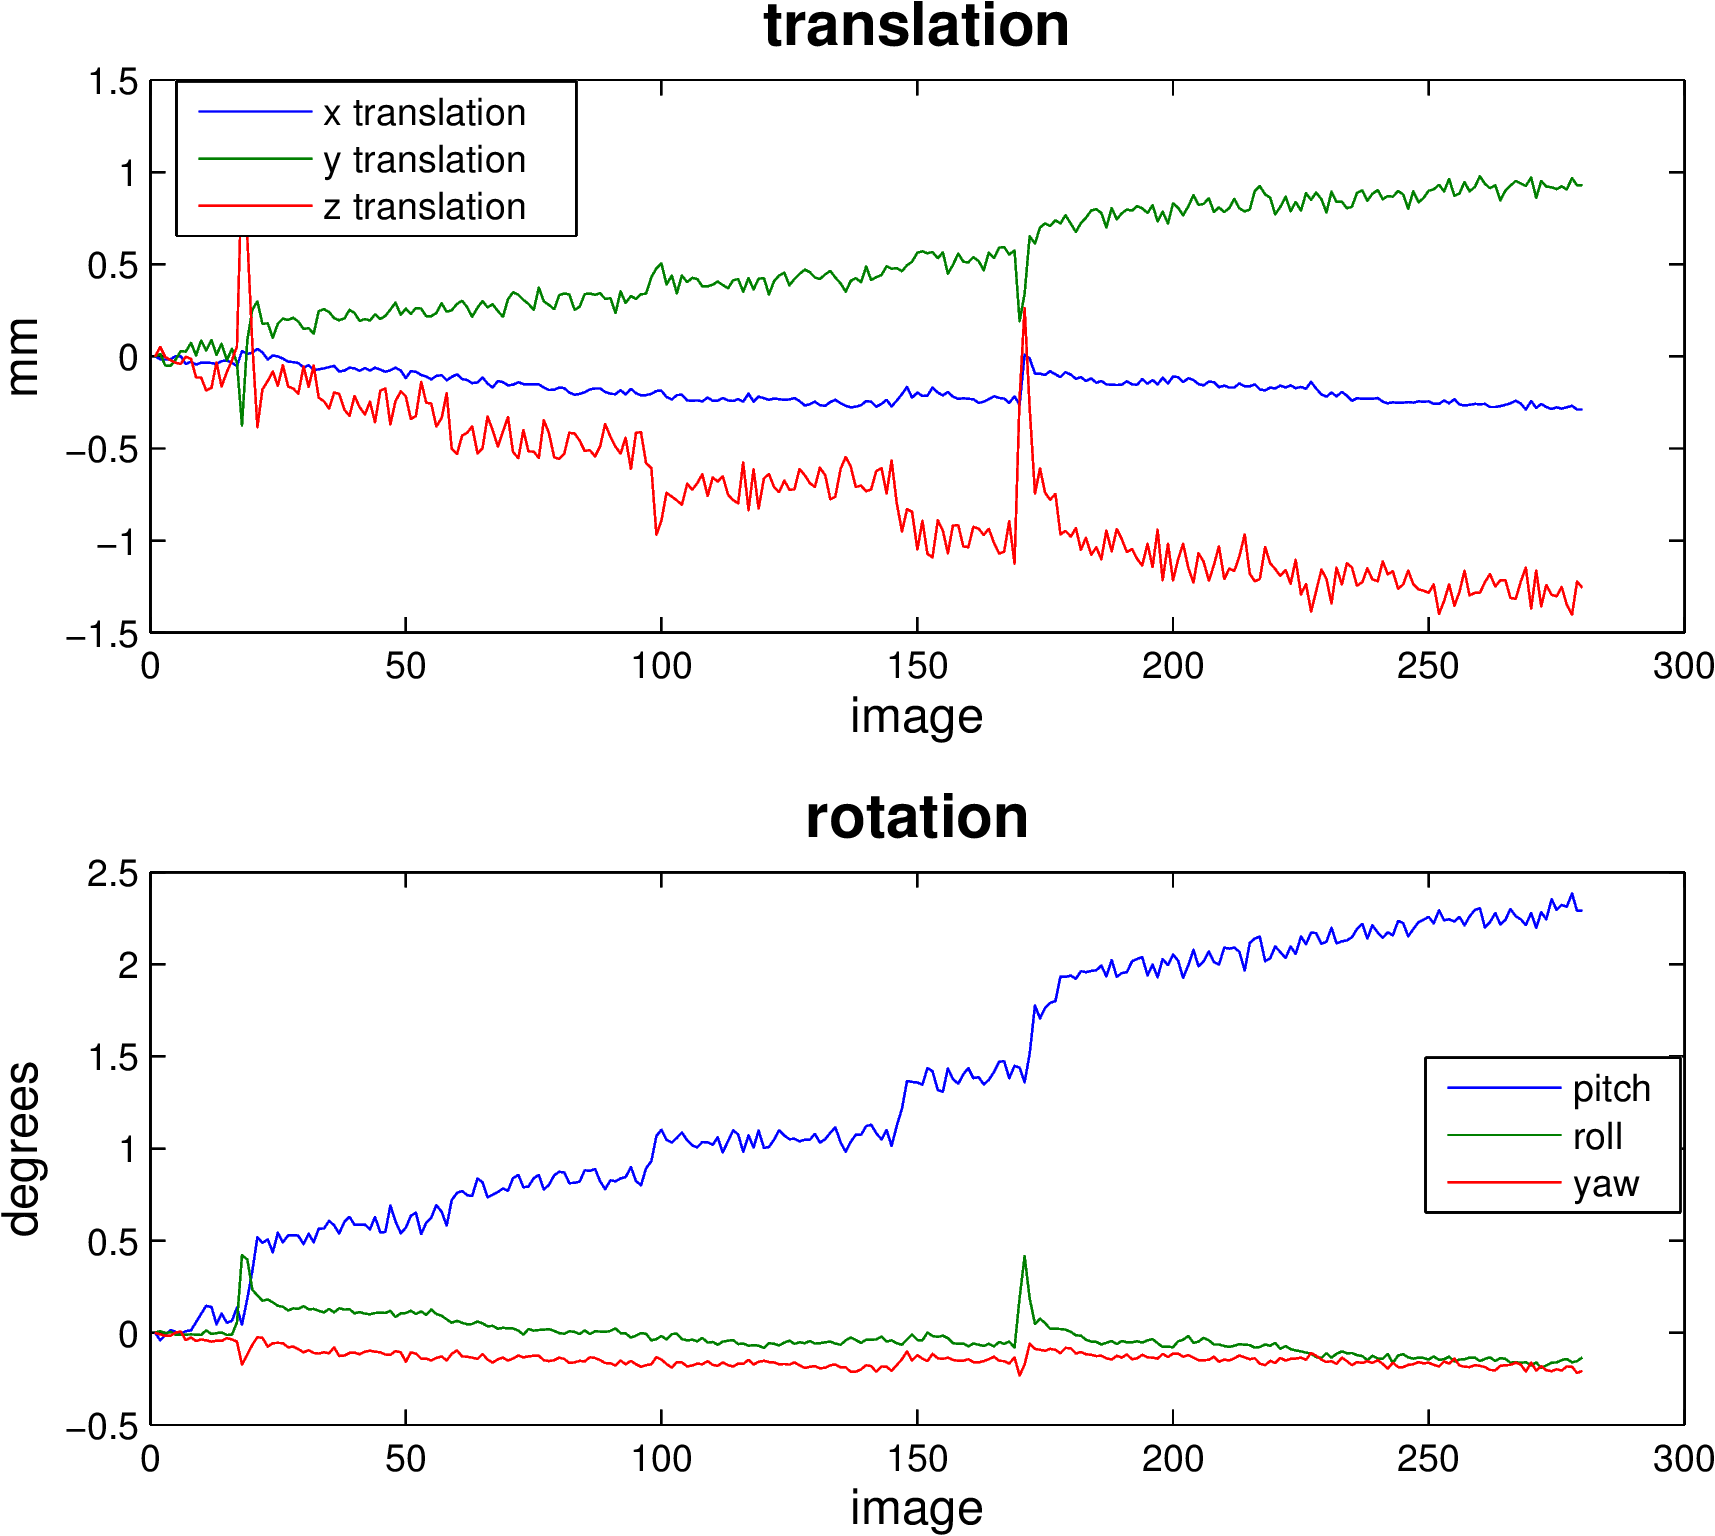
\includegraphics[scale=0.15]{img/arts.png}
  \caption{Artefactos}         \label{preproc:arts}
\end{figure}

El preproceso de corrección de movimiento intenta corregir los movimientos más pequeños, no obstante a veces es mejor simplemente eliminar los volumenes que han sido adquiridos durante el movimiento extremo. La detección de artefactos se utiliza a fin de identificar estos volumenes para que sean eliminados en fases posteriores del análisis.

\subsection{Registro basado en una template}

Los usos más comunes de esta etapa del preprocesado son:
\begin{itemize}
	\item Combinar diferentes sujetos en un grupo de estudio 
	\item Corrección del movimiento
	\item Cuantificar cambios estructurales
\end{itemize}

\subsubsection{Tipos de registro de imagen}

\begin{itemize}
	\item Según la complejidad en grados de libertad (df)
	\begin{itemize}
		\item Cuerpos rígidos $(6 df)$
		\item Affine $(12 df)$
		\item No-lineal $(>12 df)$
	\end{itemize}
	\item Normalización (la misma persona)
	\begin{itemize}
		\item Sección cruzada (cross-sectional) entre diferentes modalidades de imagen.
		\item Longitudinal en la misma modalidad entre dos visitas distintas
		\item Longitudinal entre diferentes modalidades y distintas visitas.
	\end{itemize}
	\item Normalización: registrar en una template, por ejemplo MNI152 T1.
	\item Un sujeto en otro distinto
\end{itemize}

\paragraph{El registro lineal} es el más simple. Tiene 6 grados de libertad y consisten en traslación y rotación: $$T_{rigid}(v) = Rv + t$$
Donde $v$ es un voxel en el epacio en 3D, esencialmente una matriz de rotación $R$ múltiplica el voxel $v$ y suma la traslación $t$. En otras palabras se obtiene la imagen, se rota y se traslada. Esta es una transformación de cuerpo rígido.

\begin{figure}[H]
  \centering
    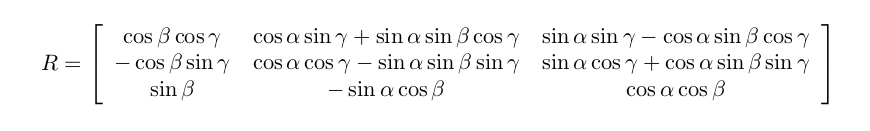
\includegraphics[scale=0.5]{img/rotation.png}
  \caption{Matriz de rotación}         \label{preproc:matriz_rot}
\end{figure}

\begin{figure}[H]
  \centering
    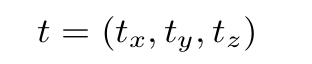
\includegraphics[scale=0.5]{img/tras_vec.png}
  \caption{Vector de traslación}         \label{preproc:tras_vec}
\end{figure}

Existen $6$ grados de libertad ya que hay 3 ángulos de rotación y 3 posibles ejes de traslación $x,y,z$. 

\paragraph{El registro lineal afín.} La transformación afín tiene 12 grados de libertad. De la misma forma que la rígida, pero la matriz $A$ no se limita a una matriz de rotación, todos los valores pueden ser distintos en cada posición, no existen restricciones.
Es por esto que la matriz de transformación afín $A$ tiene 9 campos (una matriz de $3x3$) y el vector de traslación $3$, en total $12$ grados de libertad.
El vector de traslación es exactamente el mismo que el de la transformación de cuerpo rígido.
$$T_{affine}(v) = Av + t$$

Estás dos transformaciones lineales son las más utilizadas. 

\begin{figure}[H]
  \centering
    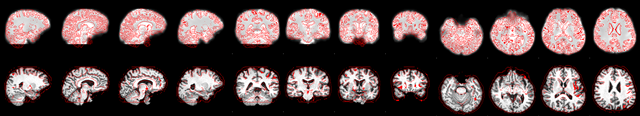
\includegraphics[scale=0.75]{img/func2t1.png}
  \caption{Registro de una imagen funcional en una imagen T1 del mismo individuo}         \label{preproc:func2t1}
\end{figure}

\paragraph{Normalización}. Se obtienen mejores resultados con un menor número de grados de libertad. Esto es debido a que se trata del mismo cerebro, y por tanto no es necesario realizar grandes transformaciones para registrar un cerebro utilizando otro distinto.
Algunos ejemplos de análisis que no requieren plantillas de referencia ya que es suficiente con co-registrar las imágenes:
\begin{itemize}
 \item Identificar cambios longitudinales específicos de la ubicación: cambios en un mismo cerebro para diferentes visitas. Es decir, que ha cambiado en un cerebro en particular.
 \item Segmentación. Suponiendo que estamos interesados en identificar la materia blanca, gris o el area correspondiente a una patología no es necesario utilizar una template. Es posible realizarlo y existen métodos relacionados, sin embargo no es necesario.
 \item Análisis de intensidades.
\end{itemize}

Existen muchos otros ejemplos en los que no es necesario aplicar esta técnica de preprocesado. Conviene evitarlo si es posible, aunque existen contextos en los que es necesario registrar las imágenes utilizando una \textbf{template}.

\begin{figure}[H]
  \centering
    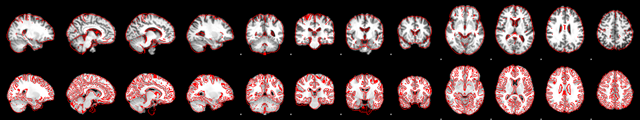
\includegraphics[scale=0.75]{img/highres2mni.png}
  \caption{ Registro T1 en una template MNI}         \label{preproc:highres2mni}
\end{figure}

\paragraph{ Registro basado en una template.} Asume que el cerebro puede ser manipulado en un espacio muestral dada una plantilla. A menudo está cuestión es motivo de debate. No siempre es razonable por que el cerebro es una estructura muy compleja.
Se obtiene información anatómica de la plantilla, por ejemplo para poder identificar las regiones del cerebro.
Ejemplos de análisis que requieren utilizar esta técnica:
\begin{itemize}
	\item Para obtener resultados de una población (p. e. localización de lesiones)
	\item Describir hallazgos a nivel anatómico
	\item Segmentación utilizando un multi-atlas. Obtener información del diferentes template de atlas cerebrales.
\end{itemize}

\subsection{Suavizado}

Más comunmente conocido por el termino en inglés smoothing. Se trata de aplicar un filtro a la imagen. Al suavizar una imagen se incrementa el \hyperref[glos:snr]{SNR} de los datos filtrando las frecuencias más altas en el dominio de la frecuencia. Dicho de otra forma, elimina los cambios más pequeños de escala entre los voxels. Esto ayuda a que los cambios a mayor escala sean más evidentes. 
Existe una cierta variabilidad inherente en la localización funcional entre sujetos y por tanto suavizar ayuda a minimizar las diferencias espaciales entre sujetos y por esto es importante aplicar el filtro en estudios de grupos de sujetos. \\

\begin{figure}[H]
 \centering
    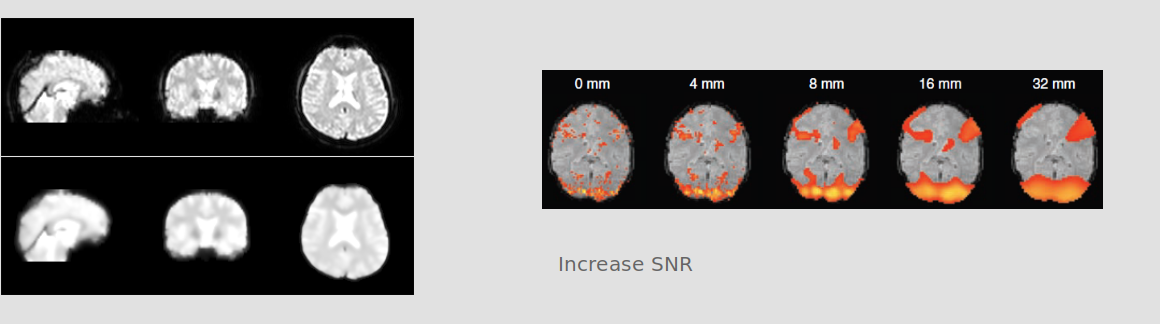
\includegraphics[scale=0.35]{img/smooth.png}
  \caption{Suavizado con diferentes parámetros de filtro}         \label{preproc:smooth}
\end{figure}

El suavizado se implementa aplicando un Kernel gausiano 3D a la imagen, la cantidad de suavizado se determina por su anchura total establecido en el parámetro medio máximo (fwhm). Este parámetro indica el diametro del núcleo de suavizado. El valor de cada voxel se cambia como resultado de aplicar este kernel de suavizado a su valor original. Para el valor de este parámetro algunos autores sugieren usar dos veces las dimensiones de voxel como un punto de partida razonable.\cite{brainhack}


%%=========================================
\section{Redes cerebrales}
 
El campo de las matemáticas que describe y cuantifica las redes se denomina teoría de grafos.
 
 \begin{figure}[H]
  \centering
    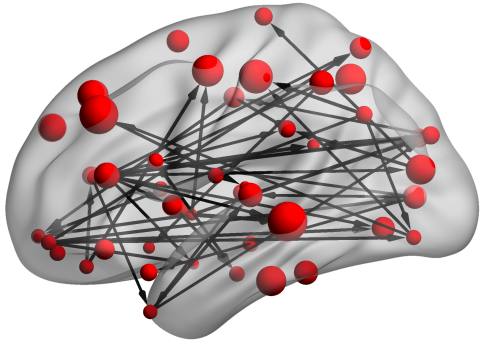
\includegraphics[scale=0.5]{img/net.png}
  \caption{Red de conectividad cerebral}         \label{preproc:net}
\end{figure}
%%%=========================================

Para construir un grafo primero se seleccionan los nodos que constituiran el grafo. Una vez hecho esto es necesario definir la conectividad entre las distintas regiones del cerebro. Los nodos representan las regiones de interés del cerebro.

Existen distintas técnica con el fin de seleccionar los nodos:

\begin{itemize}
	\item Basada en los voxel: Cada voxel de la imagen es usado como el vertice del grafo.
	\item Basado en un atlas: Se definen los nodos por el conocimiento anatómico del cerebro.
	\item Basado en los datos: Los nodos son definidos basandose en los datos extraidos de las imágenes MRI.
\end{itemize}

La conectividad cerebral se puede clasificar según su naturaleza:

\begin{itemize}

	\item Conectividad anatómica: decodifica las conexiones cerebrales anatómicas, estas conexiones tipicamente son traceadas por la materia blanca (WM).
	\begin{figure}[H]
  		\centering
    	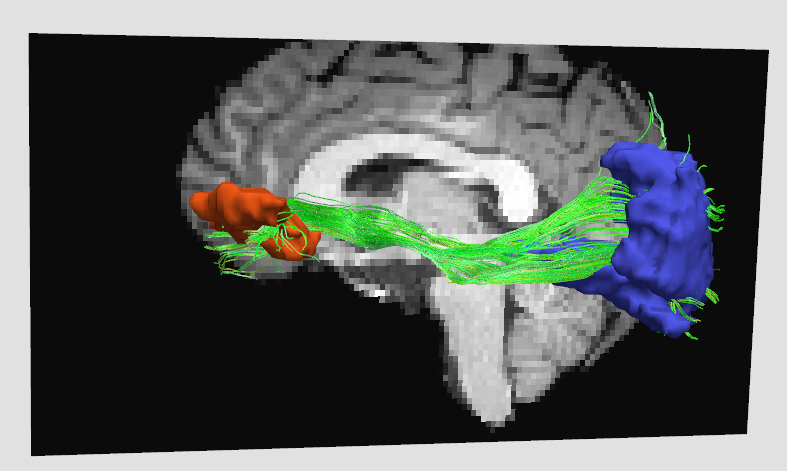
\includegraphics[scale=0.5]{img/anat_conect.png}
  		\caption{Conectividad anatómica}         \label{preproc:anat_conect}
	\end{figure}
	
	Las medidas utilizadas para el cálculo de la conectividad funcional son:
	\begin{itemize}
		\item Numero de fibras
		\item Volumen
		\item Densidad
		\item Longitud de las fibras
		\item Anisotropía fraccional
		\item Ratio de difusión media
		\item Ratio de difusión radial
		\item Ratio de difusión axial
	\end{itemize}
	
	\item Conectividad funcional: define los distintos patrones de activación entre las distintas poblaciones de neuronas. Los nodos con actividad funcional similar están conectados.
	
	\begin{figure}[H]
  		\centering
    	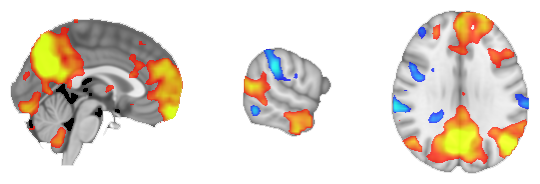
\includegraphics[scale=0.5]{img/func_conect.png}
  		\caption{Conectividad funcional}\label{preproc:func_conect}
	\end{figure}
	
	Las medidas utilizadas para el cálculo de la conectividad funcional son:
	\begin{itemize}
		\item Correlación de Pearson
		\item Correlación Parcial
		\item Información mutua
		\item Coherencia
		\item Sincronización de fase
		\item Sincronización no lineal generalizada
	\end{itemize}
	
	\item Conectividad efectiva: identifica interacciones causales subrayando la activación en orden temporal de activación o el flujo de información.
	
	\begin{figure}[H]
  		\centering
    	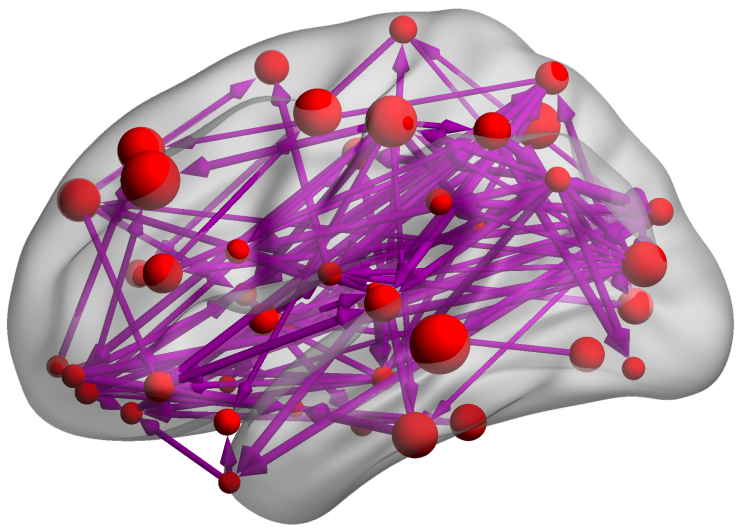
\includegraphics[scale=0.5]{img/eff_conect.png}
  		\caption{Conectividad efectiva: La conectividad efectiva es una medida dirigida mientras que la conectividad funcional y estructural no lo son}         \label{preproc:eff_conect}
	\end{figure}	
	
	Las medidas que proveen las redes efectivas de conectividad son:
	\begin{itemize}
		\item Causalidad de Granger
		\item Entropía de transferencia
		\item Modelado causal directo
		\item Modelado de equación estructural
	\end{itemize}
	
\end{itemize}
\cite{brainhack}.

Una puede ser representada mediante su matriz de conectividad

	\begin{figure}[H]
  		\centering
    	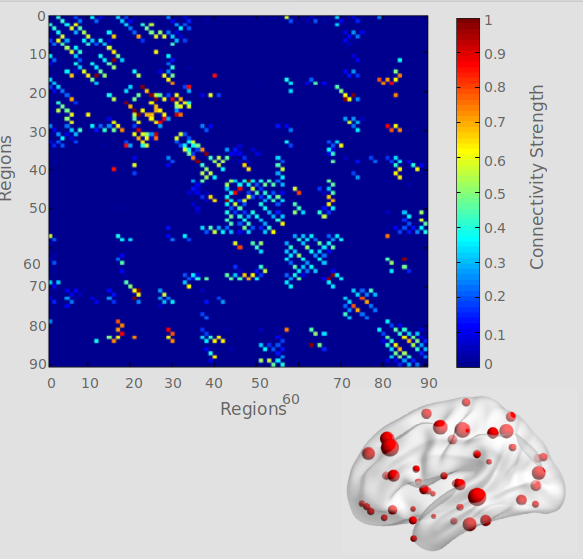
\includegraphics[scale=0.5]{img/matrix_conect.png}
  		\caption{Matriz de conectividad}         \label{preproc:matrix_conect}
	\end{figure}
	
En la matriz \ref{preproc:matrix_conect} podemos observar que el nodo 52 y el nodo 3 no están conectados, dicho de otra forma el valor en la matriz es 0. Sin embargo el nodo 79 se encuentra fuertemente conectado con el 3.

\section{Análisis no lineal}

 Desde 1994 el modelo lineal general (GLM) se ha convertido en la herramienta principal de análisis fMRI debido a su flexibilidad para incorporar múltiples variables independientes cualitativas y cuantitativas. El propósito del GLM, es predecir la variación de una variable dependiente en terminos de una combinación lineal (suma ponderada) de las variables explicativas. El análisis estandar de datos fMRI se basa en rl snślidid masivo univariante. El modelo se estima para cada voxel de forma independiente.
 
 	\begin{figure}[H]
  		\centering
    	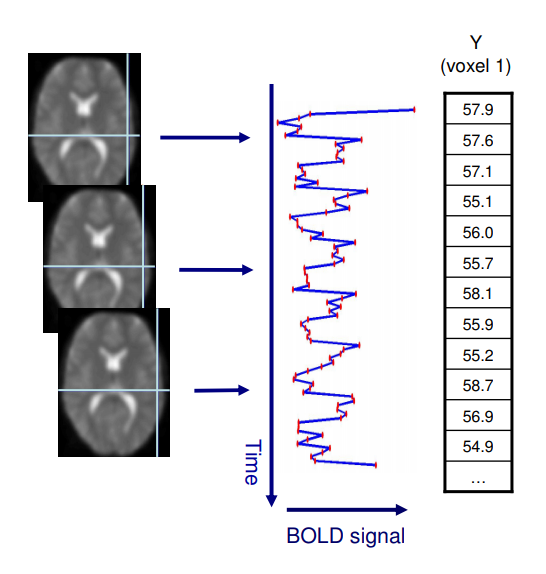
\includegraphics[scale=0.5]{img/glm.png}
  		\caption{}         \label{preproc:glm}
	\end{figure}

$Y$ es un vector que recoge la señal \textbf{BOLD} de un único voxel en volumenes sucesivos.
	
 Las imágenes obtenidas por fMRI no son estacionarias pueden ser modeladas con técnicas no lineales dado su bajo coste computacional y por representar soluciones confiables. 

-Introducción a las técnicas lineales
-Justificación uso de medidas no lineales
-Uso de técnicas no lineales
%	1.Metodos no parametricos
%	2.Metodos parametricos
%	3.Metodos tiempo frecuencia